\documentclass[conference]{IEEEtran}
\usepackage{amsmath,amssymb,booktabs,graphicx,tikz}
\usetikzlibrary{arrows.meta,positioning,fit,backgrounds}
\usepackage[hidelinks]{hyperref}
\providecommand{\AnalysisPath}{../../results/analysis}
\providecommand{\TracePath}{../../results/visualization}
\graphicspath{{\AnalysisPath/}{\TracePath/}}
\input{\AnalysisPath/numbers.tex}
\hypersetup{pdftitle={Systolic Array Scaling Under Modeled Input Bandwidth Limits},pdfauthor={Ozlem Polat, Thomas Martin, Keith Kamer}}
\title{Systolic Array Scaling Under Modeled Input Bandwidth Limits}
\author{\IEEEauthorblockN{Ozlem Polat, Thomas Martin, and Keith Kamer}\IEEEauthorblockA{University of Florida}}
\setcounter{dbltopnumber}{3}
\renewcommand{\dbltopfraction}{.95}
\renewcommand{\dblfloatpagefraction}{.8}
\renewcommand{\textfraction}{.05}
\begin{document}
\maketitle
\begin{abstract}
We evaluate an output-stationary VHDL matrix multiplier across three processing-element grids, two matrix orders, and three modeled operand-supply budgets. The study contains \SimulationCases{} passing numerical cases over \SimulationConfigurations{} configurations and \HardwareConfigurations{} post-route FPGA implementations for order-16 matrices. At full input supply, order-16 products require \ComputeLargeTwo{}, \ComputeLargeFour{}, and \ComputeLargeEight{} compute clocks on the three grids. The largest grid achieves a \WideSpeedup{}-fold compute speedup over the 2-by-2 grid with sixteen times the processing elements. Restricting its input budget to four words introduces \LimitedStalls{} stalls and raises compute latency to \LimitedCompute{} clocks. Useful utilization is \WideUtilization{}\% at full supply, reflecting finite-workload fill/drain and capture costs. Serial readout reduces the largest grid's complete-product speedup to \LargeEndSpeedup{}. All three FPGA implementations meet the constrained internal 10 ns target. The largest grid minimizes latency, while the smallest provides the highest useful throughput per DSP. These results quantify distinct limits from operand supply, finite-workload scheduling, and result delivery.
\end{abstract}
\begin{IEEEkeywords}
systolic array, matrix multiplication, input bandwidth, FPGA, architectural evaluation, reproducibility
\end{IEEEkeywords}

\section{Introduction}
Systolic matrix accelerators distribute multiply-and-accumulate (MAC) work across a regular grid. Increasing the grid dimension raises peak arithmetic capacity, but useful performance also depends on operand delivery, finite-workload scheduling, and result handling. A comparison based only on PE count can therefore miss the main costs of a complete implementation.

This study asks how array size and a controlled input budget affect a complete matrix product. We use one output-stationary VHDL design with square PE grids $P\in\{2,4,8\}$, matrix orders $N\in\{8,16\}$, and combined boundary-input budgets $B\in\{4,8,16\}$ words per clock. Each configuration performs the same dense product for its matrix order. The 2-by-2 grid supplies the architectural reference.

The experiments test two hypotheses. First, constrained input supply reduces the scaling efficiency of larger arrays. Second, short products retain substantial fill/drain overhead even at full supply. A further implementation question is whether reduced latency justifies additional FPGA resources. We measure serial readout separately so compute speedup is not confused with complete-product speedup.

The contribution is a controlled RTL study with complete-product verification, a cycle-accounting model checked against observed events, and measured FPGA implementation evidence. The input budget models the RTL boundary interface. It does not measure KV260 DRAM bandwidth or system-level accelerator performance.

\section{Related Work}
The TPU study establishes a large matrix-multiply array as a practical inference substrate and shows the importance of data delivery to utilization~\cite{tpu}. SCALE-Sim exposes array shape, dataflow, and bandwidth parameters for cycle-level accelerator exploration~\cite{scale}. These studies motivate varying arithmetic capacity and operand supply together.

Gemmini evaluates accelerator configurations within a complete hardware/software stack~\cite{gemmini}. Its scope includes effects that our isolated RTL experiment omits, including processor integration and software overhead. Scale-out Systolic Arrays studies array granularity, interconnect, and tiling across multiple pods~\cite{sosa}. Our experiment holds the dataflow and PE design fixed and varies only a small square grid, complete matrix workload, and modeled input supply.

Palacios et al. co-design systolic arrays with structured pruning for edge transformers, examining performance, hardware cost, and application accuracy~\cite{sasp}. Their results motivate examining costs alongside speedup. Their pruning-dependent scaling mechanism differs from our dense workload's input-supply, wavefront, capture, and readout costs; their ASIC area and energy values are not directly comparable with our FPGA resource counts.

Consequently, the findings are specific to this controller, capture schedule, arithmetic width, and input interface. They provide an inspectable explanation of measured scaling rather than a new dataflow or a universal optimum array size.

\section{Architecture}
\subsection{Dataflow and arithmetic}
Every PE receives a signed 16-bit $A$ operand from the left and a signed 16-bit matrix-$B$ operand from above. Registered links forward values and valid bits. When both operands are valid on an enabled edge, the PE accumulates their product locally:
\begin{equation}
C[i,j]=\sum_{k=0}^{N-1}A[i,k]B[k,j].
\end{equation}
The accumulator is signed 36-bit for every configuration. This preserves the exact 16-term signed-extreme sum and holds arithmetic precision constant across workloads. The standalone budget symbol $B$ is distinct from an entry of matrix $B[k,j]$.

Tile indices $(u,v)$ select global origins $(r_0,c_0)=(uP,vP)$. Operand $A[r_0+r,k]$ enters row $r$ on enabled boundary step $k+r$, while $B[k,c_0+c]$ enters column $c$ on step $k+c$. The matching pair meets at PE $(r,c)$ on enabled step $k+r+c$. Useful work remains stationary in the accumulator while operands propagate right and down.

\begin{figure*}[t]
\centering
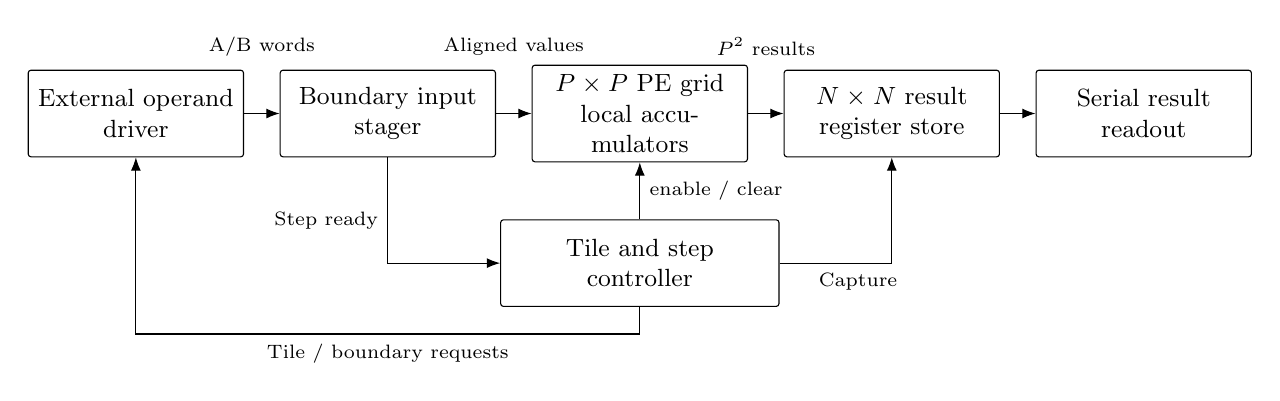
\begin{tikzpicture}[font=\small,box/.style={draw,rounded corners=1pt,align=center,minimum height=11mm,text width=25mm},>=Latex]
\node[box] (driver) at (0,0) {External operand\\driver};
\node[box] (stage) at (3.2,0) {Boundary input\\stager};
\node[box] (grid) at (6.4,0) {$P\times P$ PE grid\\local accumulators};
\node[box] (store) at (9.6,0) {$N\times N$ result\\register store};
\node[box] (read) at (12.8,0) {Serial result\\readout};
\node[box,text width=33mm] (ctrl) at (6.4,-1.9) {Tile and step controller};
\draw[->] (driver)--(stage);
\draw[->] (stage)--(grid);
\draw[->] (grid)--(store);
\node[font=\scriptsize] at (1.6,.85) {A/B words};
\node[font=\scriptsize] at (4.8,.85) {Aligned values};
\node[font=\scriptsize] at (8,.85) {$P^2$ results};
\draw[->] (store)--(read);
\draw[->] (ctrl.north)--node[right,font=\scriptsize]{enable / clear}(grid.south);
\draw[->] (stage.south)|-node[left,pos=.3,font=\scriptsize]{Step ready}(ctrl.west);
\draw[->] (ctrl.east)-|node[below,pos=.35,font=\scriptsize]{Capture}(store.south);
\draw[->] (ctrl.south)--(6.4,-2.8)--node[below,font=\scriptsize]{Tile / boundary requests}(0,-2.8)--(driver.south);
\end{tikzpicture}
\caption{Implemented data path and control. The operand driver belongs to the experimental environment. The result store and serial readout belong to the RTL. A complete boundary step enables the entire grid, preserving operand alignment across stalls.}
\label{fig:arch}
\end{figure*}

\subsection{Input staging and tiling}
The stager accepts at most $B$ new boundary words per physical clock. A partially accepted step retains its values while the grid holds. On the completing clock it bypasses unstored values directly, avoiding an extra staging clock when supply is sufficient. Empty drain steps advance without demanding operands. This implements a combined A/B-word budget rather than separate independent channel budgets.

There are $Q=(N/P)^2$ output tiles. Each tile streams the full inner dimension $N$, advances for $N+2P-2$ enabled steps, and uses one capture clock. Capture writes $P^2$ results and clears the grid. The controller then advances through output tiles in row-major order. After the final tile it serializes the complete result in $N^2$ clocks. The readout has no backpressure and assumes every valid word is consumed.

The selected mapping uses registers for the result store. Its capacity is $36N^2$ bits. A matrix order therefore changes more than the number of tiles: it changes result storage, addressing, capture selection, and readout logic. Figure~\ref{fig:arch} separates these components from the arithmetic array.

\section{Experimental Method}
\subsection{Workloads and correctness}
The Cartesian product contains \SimulationConfigurations{} simulation configurations. Each runs eight cases: zero, identity, two signed-extreme cases, mixed signs, and three fixed-seed random cases. A Python reference computes exact full-width matrix products. Canonical vector files and SHA-256 manifests identify the input bytes.

The QuestaSim 2026.2 sweep passes all \SimulationCases{} cases. The committed independent GHDL 5.0.1 sweep also passes all cases and reproduces the simulation-summary counters~\cite{ghdl}. Every result word is checked at full width, together with readout order, exact $N^3$ useful MACs, and independent interface-clock observations. The analysis checks each configuration against the cycle model rather than validating only a single representative row.

Directed regressions cover PE reset/clear priority, valid forwarding, global holds, partial input staging, and agreement between instrumented and synthesis-mode outputs. This synthesis-mode comparison is a directed simulation regression. Activity traces record all configurations and validate contiguous clocks, zero MAC events during stalls, $N$ useful MACs per PE before each tile capture, and complete tile counts. Figure~\ref{fig:verify} summarizes the verification and reporting workflow.

\begin{figure}[t]
\centering
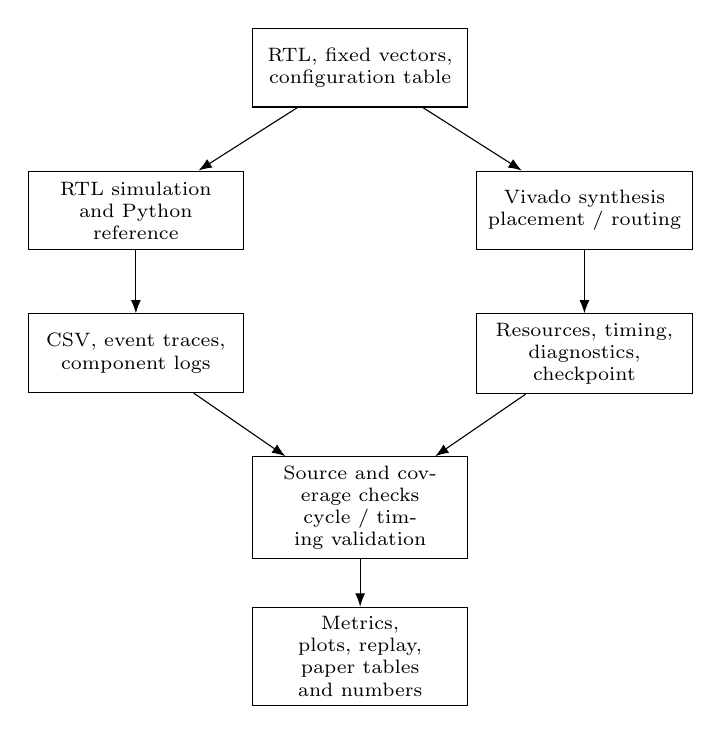
\begin{tikzpicture}[font=\scriptsize,>=Latex,node distance=6mm,box/.style={draw,align=center,text width=25mm,minimum height=10mm}]
\node[box] (source) {RTL, fixed vectors,\\configuration table};
\node[box,below left=8mm and 1mm of source] (sim) {RTL simulation\\and Python reference};
\node[box,below right=8mm and 1mm of source] (fpga) {Vivado synthesis\\placement / routing};
\node[box,below=8mm of sim] (trace) {CSV, event traces,\\component logs};
\node[box,below=8mm of fpga] (reports) {Resources, timing,\\diagnostics, checkpoint};
\node[box,below right=8mm and 1mm of trace] (validate) {Source and coverage checks\\cycle / timing validation};
\node[box,below=of validate] (analysis) {Metrics, plots, replay,\\paper tables and numbers};
\draw[->](source)--(sim);\draw[->](source)--(fpga);
\draw[->](sim)--(trace);\draw[->](fpga)--(reports);
\draw[->](trace)--(validate);\draw[->](reports)--(validate);
\draw[->](validate)--(analysis);
\end{tikzpicture}
\caption{Verification and reporting workflow. Completed measurements pass the validation gate before becoming the selected analysis dataset.}
\label{fig:verify}
\end{figure}

\subsection{FPGA comparison}
The hardware comparison uses the saved Vivado 2025.2.1 synthesis and routed reports for $N=16$, $P\in\{2,4,8\}$, targeting \texttt{xck26-sfvc784-2LV-c}. All three builds use a 10 ns clock, out-of-context synthesis, optimization, placement, routing, one tool thread, default directives, and \texttt{INSTR=false}. The runtime input budget does not require a separate synthesis build. Each hardware result therefore pairs with the three input-budget simulations for the same grid and matrix order.

Resource counts are read from the implementation reports~\cite{amd}. Setup and hold slack and unconstrained-internal-endpoint counts are checked alongside the numerical summaries. External input/output delays are unspecified in this OOC flow. The reported timing qualifies constrained internal paths; board interface timing and physical DRAM performance are outside the measurement boundary.

\section{Cycle Model and Metrics}
Boundary step $t$ needs
\begin{equation}
w(t)=2\sum_{i=0}^{P-1}\mathbf{1}_{0\leq t-i<N}
\end{equation}
new words. The total budget-induced stall count is
\begin{equation}
S=Q\sum_{t=0}^{N+2P-3}\max\left(0,\left\lceil\frac{w(t)}{B}\right\rceil-1\right).
\end{equation}
The measured schedule follows
\begin{align}
C_c &= QN+Q(2P-2)+Q+S,\\
C_t &= C_c+N^2.
\end{align}
Here $C_c$ is compute latency and $C_t$ includes serial readout. The terms denote useful-equivalent work, fill/drain overhead, capture, and budget stalls. Since $QN=N^3/P^2$, useful-equivalent work normalizes the required MAC count by peak PE capacity. It is an accounting term; useful MACs overlap the physical fill/drain interval.

Useful throughput and PE utilization are
\begin{align}
T_{\rm MAC}&=N^3/C_c, & U&=N^3/(P^2 C_c).
\end{align}
For a fixed matrix size and budget, $S_c=C_c(P=2)/C_c(P)$, $S_t=C_t(P=2)/C_t(P)$, and scaling efficiency $\eta=S_c/(P^2/4)$. The definitions separate compute scaling from complete-result delivery.

At $f=100$ MHz, an implementation meeting internal setup and hold timing has the conditional compute rate $fN^3/C_c$. Dividing by $10^9$ gives GMAC/s. Replacing $C_c$ with $C_t$ includes readout. One MAC counts as a multiplication plus an addition, so GOP/s is twice GMAC/s. These are rates calculated from measured cycles and a timing-qualified target, not measured board rates.

\begin{table*}[t]
\centering\small
\caption{All eighteen simulation configurations. $C_c$ is compute latency, $C_t$ includes serial readout, and $S$ counts budget stalls. $S_c$/$S_t$ are speedups over the matching 2-by-2 grid; $\eta$ is PE-count scaling efficiency.}
\input{\AnalysisPath/simulation_table.tex}
\label{tab:sim}
\end{table*}

\section{Measured Scaling}
\subsection{Matrix size and input supply}
Table~\ref{tab:sim} presents every configuration. Figure~\ref{fig:combined} exposes the substantial absolute difference between complete order-8 and order-16 products. A similar curve shape does not mean equal clock counts. Additional matrix-specific latency panels are available with the generated analysis.

For $N=16,B=16$, compute latency falls from \ComputeLargeTwo{} to \ComputeLargeFour{} and \ComputeLargeEight{} clocks. The largest grid achieves \WideSpeedup{} times the compute speedup, compared with sixteen times the PE count. Its \WideEfficiency{}\% scaling efficiency quantifies the gap from ideal scaling.

For $N=16,P=8$, reducing $B$ from sixteen to four increases compute latency from \WideCompute{} to \LimitedCompute{} clocks, with \LimitedStalls{} budget stalls and a \LimitedPenalty{}-fold latency penalty. Enabled-step and capture counts remain fixed, isolating the modeled input-supply cost. A larger grid remains faster throughout the measured sweep, including the smallest budget. The results show reduced proportional benefit rather than a demonstrated scaling plateau.

\begin{figure*}[t]
\centering\includegraphics[width=.85\textwidth]{latency_combined.png}
\caption{Both matrix sizes on a shared clock axis. Solid lines denote order-16 products and dashed lines order-8 products. The axis includes the largest observed latency.}
\label{fig:combined}
\end{figure*}

\subsection{Utilization and finite-workload overhead}
Figure~\ref{fig:util} plots utilization rather than leaving it implicit in the tables. At $N=16,P=8,B=16$, useful utilization is \WideUtilization{}\%. The product uses \WideUseful{} useful-equivalent clocks, \WideFillDrain{} fill/drain clocks, and \WideCapture{} capture clocks. These structural terms explain idle capacity even without budget stalls.

At $N=8,P=8$, a single output tile still incurs the wavefront fill and drain cost. Increasing supply cannot remove that cost. Figure~\ref{fig:cycles} distinguishes structural overhead from the additional waits caused by the budget. Scaling efficiency and utilization answer different questions: efficiency normalizes speedup against the 2-by-2 reference, while utilization normalizes useful work against the candidate's own capacity.

\begin{figure*}[t]
\centering\includegraphics[width=.95\textwidth]{utilization.png}
\caption{Useful PE utilization across all grids, matrix workloads, and input budgets. Both panels use a common percentage scale.}
\label{fig:util}
\end{figure*}
\begin{figure*}[t]
\centering\includegraphics[width=.95\textwidth]{cycle_breakdown.png}
\caption{Capacity-normalized compute-cycle decomposition. Useful MACs overlap fill/drain in physical time; the stacked terms account for total capacity cost.}
\label{fig:cycles}
\end{figure*}

\subsection{Serial readout and timed throughput}
The order-8 wide-grid product requires \SmallWideCompute{} compute clocks but \SmallWideTotal{} total clocks. Serializing its \ReadoutSmall{} outputs limits end-to-end speedup to \SmallEndSpeedup{} times the 2-by-2 grid. For order-16 full-supply products, the largest grid's compute speedup is \WideSpeedup{}, but end-to-end speedup is \LargeEndSpeedup{} after \ReadoutLarge{} readout clocks.

Table~\ref{tab:sim} reports compute and end-to-end speedup and scaling efficiency for all eighteen configurations. Table~\ref{tab:eff} gives timing-qualified GMAC/s for the nine order-16 grid/budget pairs. Those rates pair each simulated workload with its measured FPGA implementation and exclude external transfers, software overhead, and intervals between products.

Figure~\ref{fig:speedup} directly compares compute and readout-inclusive scaling with PE-count scaling. Every speedup uses the matching 2-by-2 RTL workload and input budget as its denominator. No CPU measurement is available, so these curves do not imply CPU-relative acceleration. The widening gap after serial readout shows the cost of a result interface that does not scale with the grid.

\begin{figure*}[t]
\centering\includegraphics[width=.86\textwidth]{speedup.png}
\caption{Speedup relative to the 2-by-2 RTL grid at the same matrix size and input budget. Dashed gray lines show PE-count scaling, not a predicted measured result. Right-hand panels include the serial readout.}
\label{fig:speedup}
\end{figure*}

\begin{table}[t]
\setlength{\tabcolsep}{4.5pt}
\centering\small
\caption{Order-16 compute/end-to-end speedup, scaling efficiency, and conditional throughput at 100 MHz. One MAC represents two arithmetic operations. Subscripts $c$ and $t$ distinguish compute-only and readout-inclusive rates.}
\input{\AnalysisPath/efficiency_table.tex}
\label{tab:eff}
\end{table}

\section{FPGA Implementation Results}
Table~\ref{tab:fpga} places the three grid sizes side by side. Its simulation rows cover both matrix orders; hardware resources and clock-based rates refer to the order-16 builds. Figure~\ref{fig:resources} presents the implementation resources separately.

The 2-by-2, 4-by-4, and 8-by-8 implementations use \LUTLargeTwo{}, \LUTLargeFour{}, and \LUTLargeEight{} LUTs; \FFLargeTwo{}, \FFLargeFour{}, and \FFLargeEight{} flip-flops; and \DSPLargeTwo{}, \DSPLargeFour{}, and \DSPLargeEight{} DSPs. All use zero BRAM tiles. DSP count follows PE count. LUT count peaks at the 4-by-4 grid, so the grid with the most arithmetic capacity does not consume the most LUT resources in these implementations. Resource selection therefore requires the measured LUT, FF, and DSP costs together.

The complete order-16 result store contains $36N^2=9216$ bits and maps to registers in these builds. It is present alongside the PE grid, staging logic, tile controller, capture selection, and serial readout. Consequently, FPGA cost describes the complete accelerator module rather than an isolated collection of MAC units.

\begin{table}[t]
\setlength{\tabcolsep}{4.5pt}
\centering\small
\caption{Grid-to-grid comparison at full supply ($B=16$). Simulation metrics cover both matrix sizes. Hardware costs and 100 MHz rates describe the three order-16 implementations; all use zero BRAM.}
\input{\AnalysisPath/comparison_table.tex}
\label{tab:fpga}
\end{table}
\begin{figure}[t]
\centering\includegraphics[width=\columnwidth]{fpga_resources.png}
\caption{Post-route resources for the three order-16 implementations at the same 10 ns target. DSP and LUT costs have different scaling patterns.}
\label{fig:resources}
\end{figure}

All three implementations meet the constrained internal setup and hold requirements. Setup slack is \WNSLargeTwo{}, \WNSLargeFour{}, and \WNSLargeEight{} ns. The saved reports contain no unconstrained internal endpoints. The external I/O-delay counts are 71/63, 135/67, and 263/74 input/output ports, respectively; their timing is outside this OOC comparison.

Figure~\ref{fig:dsp} pairs order-16 throughput with the corresponding implemented DSP count. At full supply the three grids provide \DSPRateLargeTwo{}, \DSPRateLargeFour{}, and \DSPRateLargeEight{} useful MACs per clock per DSP. The largest array gives the shortest compute latency; the smallest provides the highest useful throughput per DSP across all three input budgets. This is a latency-versus-arithmetic-resource trade-off, while the separate LUT and FF measurements capture the remaining implementation costs.

\begin{figure}[t]
\centering\includegraphics[width=\columnwidth]{throughput_vs_dsp.png}
\caption{Order-16 useful compute throughput versus measured DSP use, with one curve per runtime input budget.}
\label{fig:dsp}
\end{figure}

\section{Recorded Activity and Reproducibility}
Figures~\ref{fig:activity8} and~\ref{fig:activity16} show every grid/budget configuration for the two complete workloads. Rows correspond to grid dimensions and columns to budgets. The recorded useful-MAC density exposes the propagating activity front, budget-induced holds, and tile transitions. Increasing supply shortens physical execution without changing the required work.

The offline topology replay shows individual MAC events. Work surfaces track completed work per PE. First/last-MAC surfaces and space--time slices show how the valid window moves through the grid and stretches during holds. These views explain the mechanism behind the scalar metrics. Their interpolated surfaces visualize discrete samples; they do not introduce additional measurements.

The configuration table drives the measurement axes. New experiments receive unique timestamped output directories automatically. The published analysis reads the committed simulation summaries and original FPGA reports. Validation checks case coverage, source records for the independent simulation, trace consistency, report values, and timing scope before generating CSVs, plots, and manuscript values. Tables and numerical macros come from the same analysis rather than manually duplicated measurements. New measurements remain in their own directories.

\section{Limitations and Extensions}
The experiment covers small dense products and one output-stationary schedule. It does not implement structured pruning, zero skipping, alternate precisions, alternate dataflows, CPU integration, or a physical memory system. Zero-valued numerical cases still exercise the complete dense-MAC schedule. Resource counts do not establish energy or power savings.

The current result store uses many parallel tile writes and serial readout. A banked or BRAM-oriented redesign could change LUT cost, FF cost, and capture latency. Overlapping input stages or output readout could also change complete-product performance. Such changes require new RTL, comparable verification, and a new cycle model where appropriate. They are extensions rather than measurements inferred from the current design.

\section{Conclusion}
Increasing the PE grid reduces compute latency in every tested configuration, but operand-supply stalls and finite-workload overhead keep speedup below PE-count scaling. Serial readout further reduces the complete-product gain. At full supply and order sixteen, the largest grid achieves \WideSpeedup{}-fold compute speedup and \LargeEndSpeedup{}-fold end-to-end speedup over the 2-by-2 reference. All three hardware builds meet the constrained internal 100 MHz target. The largest grid minimizes clocks, while the smallest maximizes useful throughput per DSP. The combined cycle, utilization, resource, and timing measurements quantify the implementation trade-off for this accelerator and interface.

\begin{samepage}
\section*{Reproducibility}
The repository contains source, fixed vectors, the simulation and FPGA evidence, validated metrics, generated plots, editable report/presentation sources, and an offline activity replay: \url{https://github.com/OzPol/systolic-array-scaling}. The command \texttt{make analysis} generates a new analysis directory from the saved measurements. Analysis requires Python and the pinned plotting environment; rerunning the FPGA implementation additionally requires the stated Vivado installation.
\end{samepage}

\newpage
\begin{thebibliography}{8}
\bibitem{tpu} N. P. Jouppi et al., ``In-Datacenter Performance Analysis of a Tensor Processing Unit,'' in \emph{ISCA}, 2017, doi: 10.1145/3079856.3080246.
\bibitem{scale} A. Samajdar, Y. Zhu, P. Whatmough, M. Mattina, and T. Krishna, ``SCALE-Sim: Systolic CNN Accelerator Simulator,'' arXiv:1811.02883, 2018.
\bibitem{gemmini} H. Genc et al., ``Gemmini: Enabling Systematic Deep-Learning Architecture Evaluation via Full-Stack Integration,'' arXiv:1911.09925, 2019.
\bibitem{sosa} A. C. Yuzuguler et al., ``Scale-out Systolic Arrays,'' arXiv:2203.11540, 2022.
\bibitem{sasp} P. Palacios, R. Medina, J.-L. Rouas, G. Ansaloni, and D. Atienza, ``Systolic Arrays and Structured Pruning Co-design for Efficient Transformers in Edge Systems,'' in \emph{GLSVLSI}, 2025, doi: 10.1145/3716368.3735158.
\bibitem{amd} AMD, \emph{Vivado Design Suite User Guide: Design Analysis and Closure Techniques}, UG906, version 2025.2, ``Report Utilization.'' [Online]. Available: \url{https://docs.amd.com/r/2025.2-English/ug906-vivado-design-analysis/Report-Utilization}.
\bibitem{ghdl} GHDL Project, ``Invoking GHDL.'' [Online]. Available: \url{https://ghdl.github.io/ghdl/using/InvokingGHDL.html}.
\end{thebibliography}

\clearpage
\appendices
\begin{figure*}[p]
\centering
{\large\bfseries Appendix: Recorded Activity Atlas\par}\vspace{4mm}
\includegraphics[width=.96\textwidth,height=.75\textheight,keepaspectratio]{activity_matrix08.png}
\caption{Recorded activity for all nine order-8 configurations. The views include complete products rather than only the first output tile.}
\label{fig:activity8}
\end{figure*}
\begin{figure*}[p]
\centering
\includegraphics[width=.96\textwidth,height=.87\textheight,keepaspectratio]{activity_matrix16.png}
\caption{Recorded activity for all nine order-16 configurations. Restricted supply stretches the physical execution of larger grids while preserving their MAC work.}
\label{fig:activity16}
\end{figure*}
\end{document}
